% Patch 0101: dashed strokes and B* (fill + stroke, even-odd). Before it, any dash crashed txp-render (SIGTRAP:
% a stack fz_stroke_state has no room for MuPDF's flexible dash array) and B* stroked in the fill colour.
\documentclass{article}
\usepackage{tikz}
\pagestyle{empty}
\begin{document}
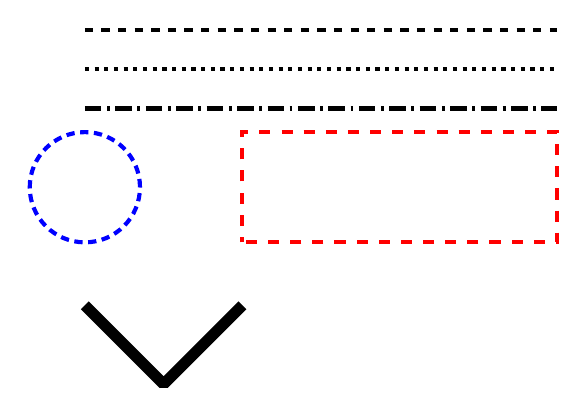
\begin{tikzpicture}[line width=1.5pt]
  \draw[dashed] (0,0) -- (6,0);
  \draw[dotted] (0,-0.5) -- (6,-0.5);
  \draw[dash pattern=on 6pt off 2pt on 1pt off 2pt] (0,-1) -- (6,-1);
  \draw[densely dashed, blue] (0,-2) circle (0.7);
  \draw[dash pattern=on 4pt off 4pt, dash phase=2pt, red] (2,-2.7) rectangle (6,-1.3);
  \draw[miter limit=1.2, line width=4pt, line join=miter] (0,-3.5) -- (1,-4.5) -- (2,-3.5);
\end{tikzpicture}

\vspace{1em}

\begin{tikzpicture}[line width=2pt]
  \draw[draw=red, fill={rgb,1:red,1;green,1}, even odd rule] (0,0) circle (1) (0,0) circle (0.5);
  \draw[draw=blue, fill=green, even odd rule, dashed] (3,0) circle (1) (3,0) circle (0.5);
\end{tikzpicture}
\end{document}
